\documentclass[12pt, a4paper]{article}  

\usepackage{amsmath,amsfonts,amssymb,amsthm,mathtools}
\usepackage{fontspec}
\setmainfont{Arial}
\usepackage{unicode-math}
\setmathfont{Asana Math}
\usepackage{polyglossia}
\usepackage{enumerate}
\setdefaultlanguage{russian}
\setotherlanguage{english}
\usepackage{graphicx}

\author{Людмила Гадий}
\title{Домашнее задание 1}
\date{\today}

\begin{document}

\maketitle

\section{10 фактов обо мне}
\begin{enumerate}
\item Безгранично люблю музыку! Пою и играю на гитаре, когда появляется свободное время.
\item Я довольно чувствительный человек.
\item Считаю, что главное в людях - искренность и жизнелюбие.
\item Стараюсь во всем искать что-то хорошее.
\item Считаю, что никогда не стоит упускать возможностей для самосовершенствования.
\item Люблю учиться чему-то новому.
\item Из двух зол выбираю сложное.
\item Мечтала стать физиком.
\item Однажды я обязательно совершу спонтанное путешествие.
\item Сова, но я стремлюсь это исправить. Сон избегает меня, Леонард!
\end{enumerate}

\section{Моя фотография}
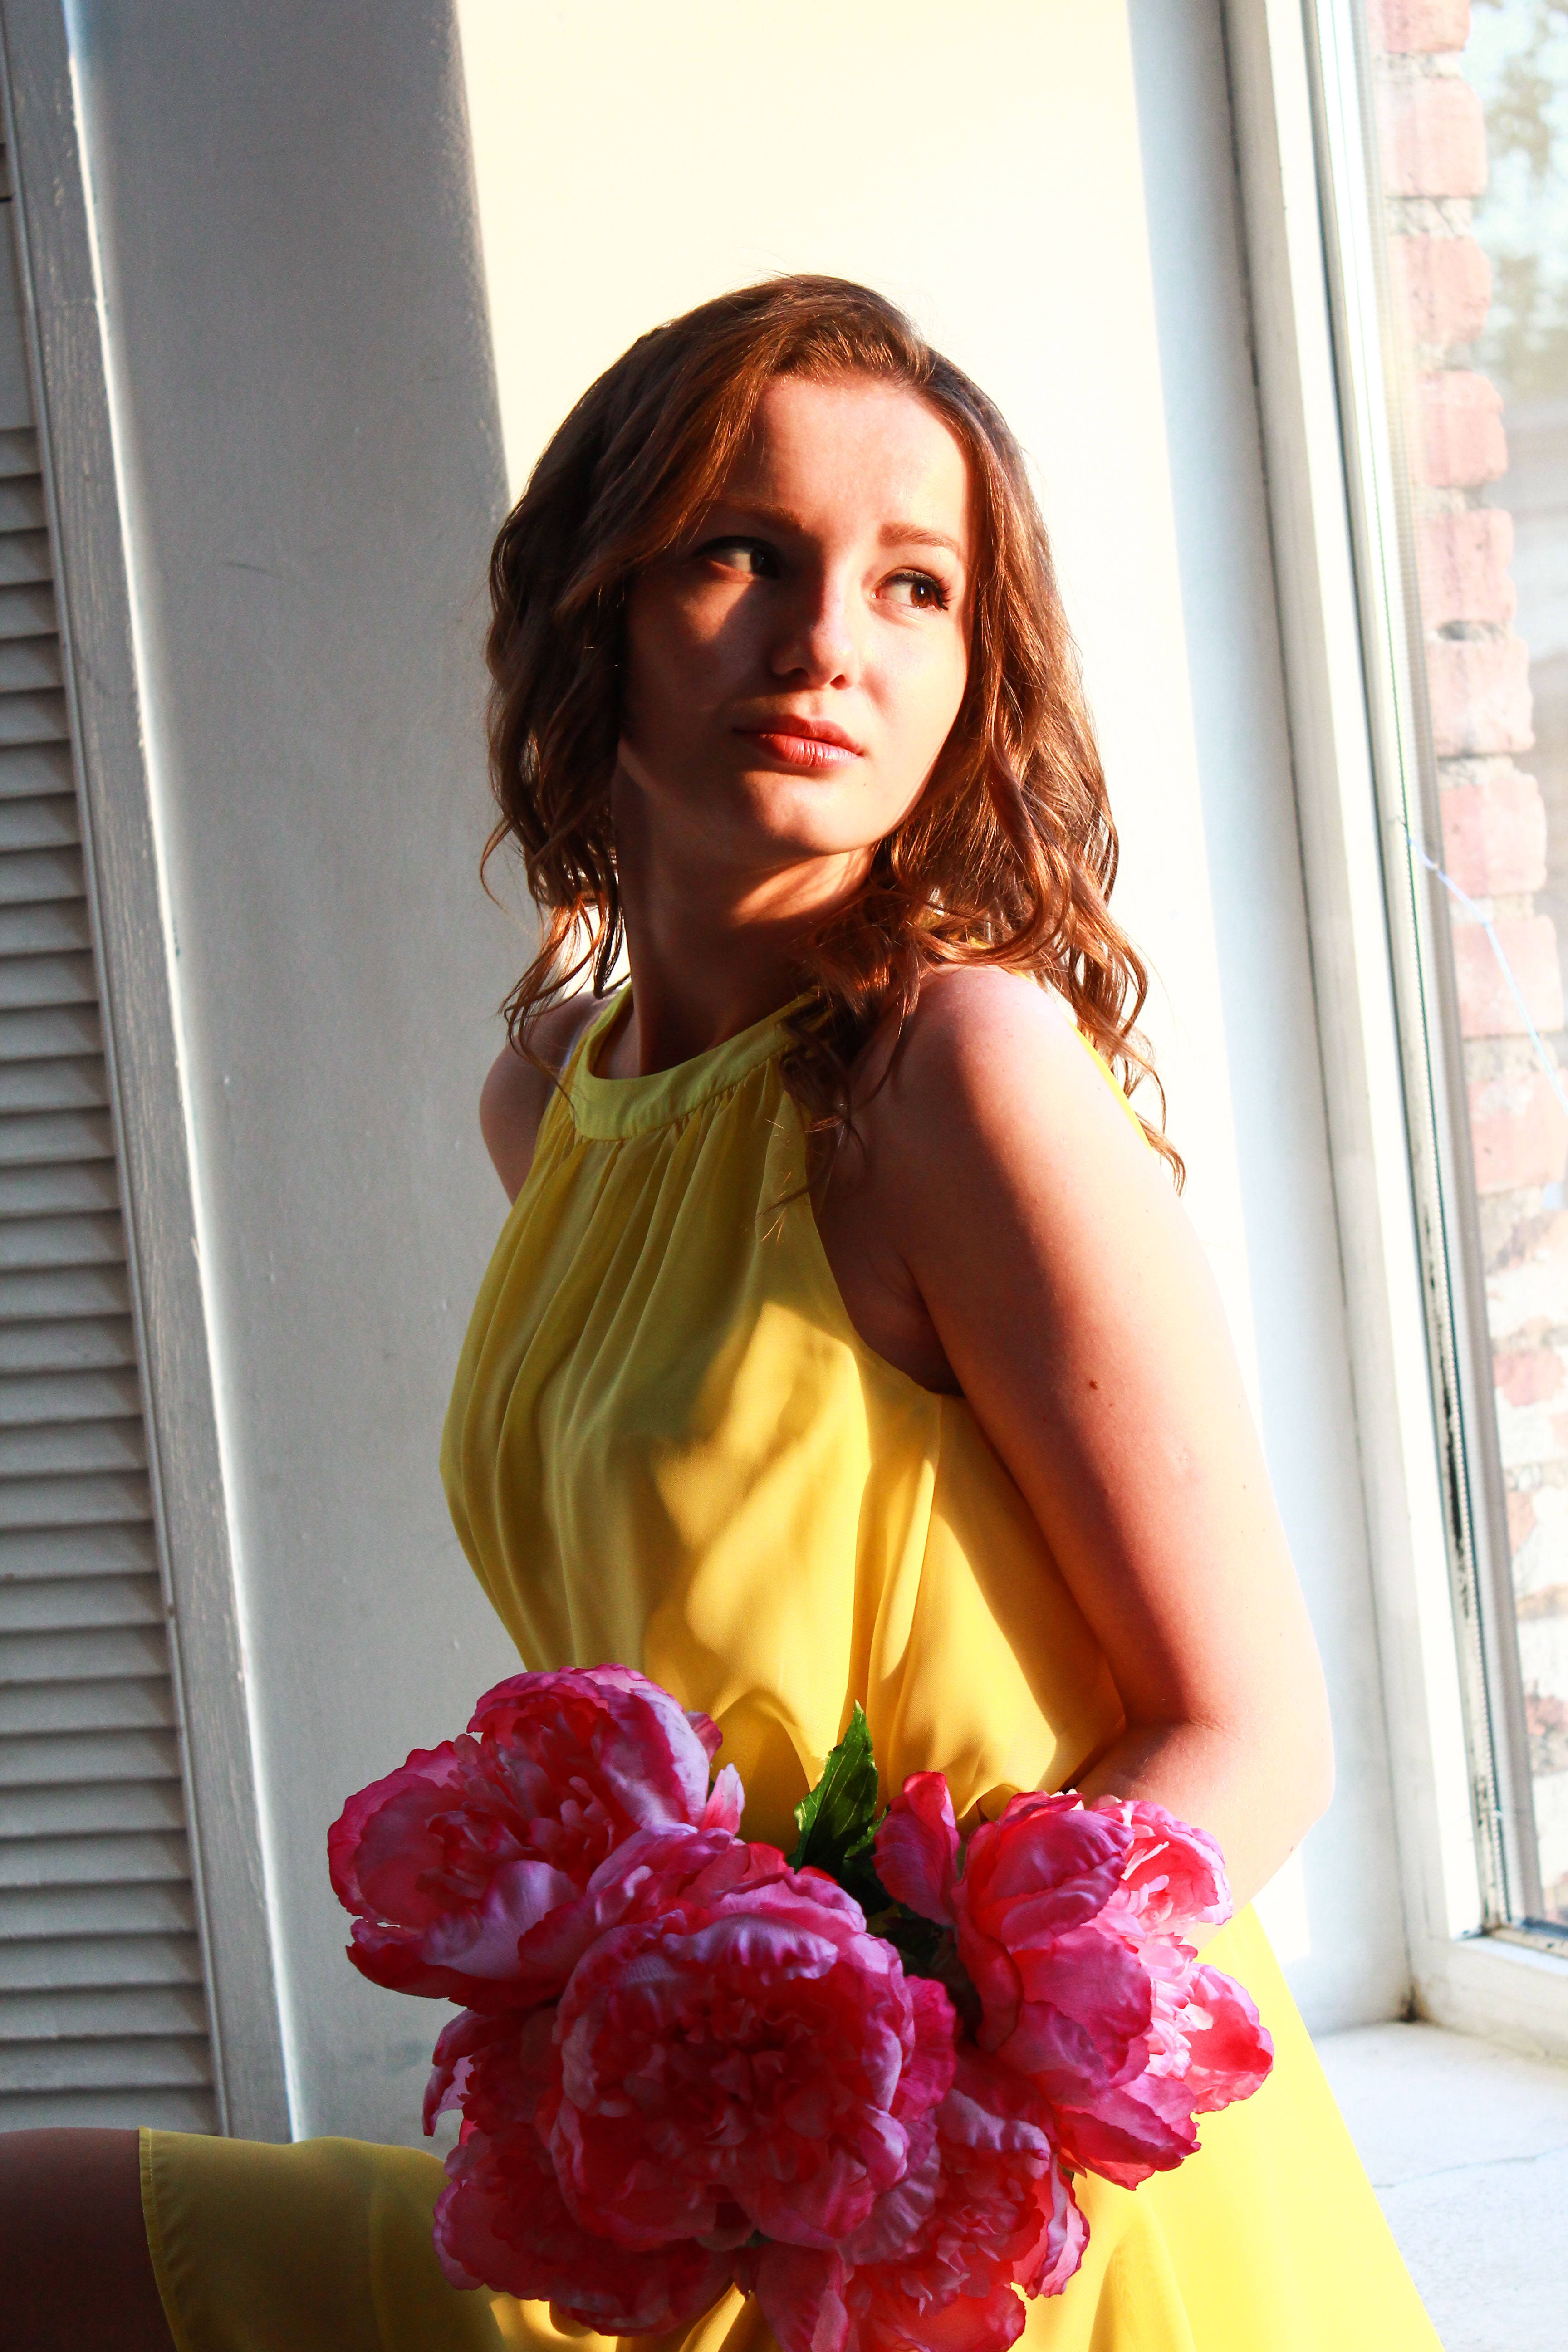
\includegraphics[scale=0.25]{MyPhoto}
\\\\\\
\section{Формулы}
\subsection{5 моих любимых формул}


Формула Стирлинга:
\begin{align*}\label{eq:Stirling}
\displaystyle \lim_{n \to \infty} \frac{n!}{\sqrt{2\pi n}*\left(\frac{n}{e}\right)^n} = 1 \tag{\ae}
\end{align*}
 Тригонометрический ряд Фурье:
\begin{align*}\label{eq:Fourier}
 \displaystyle f(x)=\frac{a_0}{2}+ \sum_{n=1}^{\infty} a_n*\cos nx + b_n*\sin nx , \tag{\ae\ae}
\end{align*}
\begin{align*}
 \displaystyle a_0=\frac{1}{\pi}\int\limits_{-\pi}^{\pi} f(x)dx , \qquad 
 \displaystyle a_n=\frac{1}{\pi}\int\limits_{-\pi}^{\pi} f(x)\cos nx dx , \qquad 
 \displaystyle b_n=\frac{1}{\pi}\int\limits_{-\pi}^{\pi} f(x)\sin nx dx .
\end{align*}
 Формула Коши-Адамара:
\begin{align*}\label{eq:Cauchy-Hadamard}
\displaystyle \rho=\frac{1}{\displaystyle \overline{\lim_{n \to \infty}} \sqrt[n]{|a_n|} }  \tag{\ae\ae\ae}  
\end{align*}
 Формула плотности двумерного нормального распределения:
\begin{align*}\label{eq:Binorm}
\displaystyle f(x,y) & = \frac{1}{\sigma_1 \cdot \sigma_2 \cdot 2\pi \cdot \sqrt{1-\rho^2}} \times{} \\
& \times \exp\left( -\frac{1}{2(1-\rho^2)} \cdot \left[\frac{(x-a_1)^2}{\sigma_1^2} + \frac{(y-a_2)^2}{\sigma_2^2}-2\rho \cdot \frac{x-a_1}{\sigma_1} \cdot \frac{y-a_2}{\sigma_2}\right]\right) \tag{\ae\ae\ae\ae}
\end{align*}
Модель линейной регрессии в матричной форме:
\begin{align*}\label{eq:LinReg}
\textbf{Y} = \pmb{\beta}\textbf{ X + U}, \tag{\ae\ae\ae\ae\ae}
\end{align*}
$ \textbf{Y} = \begin{pmatrix}
  Y_1 \\
  Y_2 \\
  \vdots \\
  Y_n
  \end{pmatrix} ,\qquad $
$ \pmb{\beta} = \begin{pmatrix}
  \beta_1 \\
  \beta_2 \\
  \vdots \\
  \beta_n
  \end{pmatrix} ,\qquad $
$ \textbf{X} = \begin{pmatrix}
  1 & X_{1,1} & \cdots & X_{1,n} \\
  1 & X_{2,1} & \cdots & X_{2,n} \\
  \vdots  & \vdots  & \ddots & \vdots  \\
  1 & X_{k,1} & \cdots & X_{k,n}
  \end{pmatrix} = 
  \begin{pmatrix}
  X'_1 \\
  X'_2 \\
  \vdots \\
  X'_n
  \end{pmatrix} ,\qquad $
$ \\\textbf{U} = \begin{pmatrix}
  u_1 \\
  u_2 \\
  \vdots \\
  u_n
 \end{pmatrix} $.


\subsection{Формула, которую мне трудно было запомнить(не могу назвать ее нелюбимой)}
Устойчивая к гетероскедастичности стандартная ошибка Эйкера-Хьюбера-Уайта для свободного члена регрессии:
\begin{align*}\label{eq:HetCons}
\displaystyle \hat\sigma_{\hat\beta_0}^2 = \frac{1}{n} \times \frac{\frac{1}{n-2} \sum \hat H_i^2\hat u_i^2}{{\left[\frac{1}{n}\sum \hat H_i^2 \right]}^2}, \qquad
\hat H_i  = 1 - \left[\frac{\overline{X}}{\frac{1}{n} \sum X_i^2} \right] \times X_i. \tag{\ae\ae\ae\ae\ae\ae}
\end{align*}


Люблю формулу \eqref{eq:Binorm}, потому что она напоминает мне о забавном случае на экзамене по теории вероятностей. Мне было трудно запомнить формулу \eqref{eq:HetCons}, потому что путалась в записи из-за ее схожести с формулой, преобразованием которой она получена.
\end{document}